\documentclass[t]{beamer}

% packages
\usepackage[english]{babel}
\usepackage[utf8x]{inputenc}
\usepackage{mathtools}
\usepackage{amsfonts}
\usepackage{amsthm}
\usepackage{numprint}
\usepackage{amsxtra}
\usepackage{amsfonts}
\usepackage{graphicx}
\usepackage{enumerate}
\usepackage{setspace}
\usepackage{booktabs}
\usepackage{tabularx}
\usepackage{amssymb, amstext, amsmath}
\usepackage{fancyhdr}

% macros
% misc
\newcommand\todo[1]{\textcolor{red}{TODO: #1}}
\newcommand\hide[1]{\textcolor{white}{#1}}

% formatting
\newcommand\bld[1]{\textbf{#1}}
\newcommand\ul[1]{\underline{#1}}
\newcommand\n[1]{\numprint{#1}}
\newcommand{\ts}{\textsuperscript}
\newcommand\red[1]{\textcolor{red}{#1}}
\newcommand\blue[1]{\textcolor{blue}{#1}}
\newcommand\link[2]{\href{#1}{\textcolor{blue}{\underline{#2}}}}

% sets
\newcommand\set[1]{\mathcal{#1}}
\newcommand\bb[1]{\mathbb{#1}}
\renewcommand\:{\colon} % for use with \sset, etc.
\newcommand{\sset}[1]{\left\{\,#1\,\right\}} % { ? }, automatic brackets
\newcommand{\ssets}[1]{\left\{#1\right\}} % {?}, automatic brackets
\newcommand{\ssetn}[1]{\{\,#1\,\}} % { ? }, normal brackets

% table formatting
% To better align bold entries in S columns (still broken)
% \usepackage{siunitx}
% \robustify\bfseries
% \newrobustcmd{\bfcell}{\bfseries}

% vector variables (taken from macros by Rainer Gemulla)
\newcommand\vect[1]{{\boldsymbol{#1}}}
\newcommand\va{\vect{a}}
\newcommand\vb{\vect{b}}
\newcommand\vc{\vect{c}}
\newcommand\vd{\vect{d}}
\newcommand\ve{\vect{e}}
\newcommand\vf{\vect{f}}
\newcommand\vg{\vect{g}}
\newcommand\vh{\vect{h}}
\newcommand\vi{\vect{i}}
\newcommand\vj{\vect{j}}
\newcommand\vk{\vect{k}}
\newcommand\vl{\vect{l}}
\newcommand\vm{\vect{m}}
\newcommand\vn{\vect{n}}
\newcommand\vo{\vect{o}}
\newcommand\vp{\vect{p}}
\newcommand\vq{\vect{q}}
\newcommand\vr{\vect{r}}
\newcommand\vs{\vect{s}}
\newcommand\vt{\vect{t}}
\newcommand\vu{\vect{u}}
\newcommand\vv{\vect{v}}
\newcommand\vw{\vect{w}}
\newcommand\vx{\vect{x}}
\newcommand\vy{\vect{y}}
\newcommand\vz{\vect{z}}
\newcommand\vzero{\vect{0}}
\newcommand\vone{\vect{1}}

\newcommand\valpha{\vect{\alpha}}
\newcommand\vbeta{\vect{\beta}}
\newcommand\veps{\vect{\epsilon}}
\newcommand\vdelta{\vect{\delta}}
\newcommand\vtheta{\vect{\theta}}
\newcommand\vsigma{\vect{\sigma}}
\newcommand\vpi{\vect{\pi}}
\newcommand\vlambda{\vect{\lambda}}

% matrix variables (taken from macros by Rainer Gemulla)
\newcommand\mA{\vect{A}}
\newcommand\mB{\vect{B}}
\newcommand\mC{\vect{C}}
\newcommand\mD{\vect{D}}
\newcommand\mE{\vect{E}}
\newcommand\mF{\vect{F}}
\newcommand\mG{\vect{G}}
\newcommand\mH{\vect{H}}
\newcommand\mI{\vect{I}}
\newcommand\mJ{\vect{J}}
\newcommand\mK{\vect{K}}
\newcommand\mL{\vect{L}}
\newcommand\mM{\vect{M}}
\newcommand\mN{\vect{N}}
\newcommand\mO{\vect{O}}
\newcommand\mP{\vect{P}}
\newcommand\mQ{\vect{Q}}
\newcommand\mR{\vect{R}}
\newcommand\mS{\vect{S}}
\newcommand\mT{\vect{T}}
\newcommand\mU{\vect{U}}
\newcommand\mV{\vect{V}}
\newcommand\mW{\vect{W}}
\newcommand\mX{\vect{X}}
\newcommand\mY{\vect{Y}}
\newcommand\mZ{\vect{Z}}
\newcommand\mzero{\vect{0}}

\newcommand{\mPi}{{\ensuremath{\vect{\Pi}}}}
\newcommand{\mSigma}{{\ensuremath{\vect{\Sigma}}}}
\newcommand{\mLambda}{{\ensuremath{\vect{\Lambda}}}}

% argmin, argmax
\DeclareMathOperator*{\argmin}{argmin} % amsmath package required
\DeclareMathOperator*{\argmax}{argmax} % amsmath package required

% matrix operations
\newcommand\xdiag{\operatorname{diag}}      
\newcommand\diag[1]{\xdiag\left(#1\right)}    % diagonal matrix


% choose how your presentation looks.
% for more themes, color themes and font themes, see:
% http://deic.uab.es/~iblanes/beamer_gallery/index_by_theme.html

\mode<presentation>
{%
	\usetheme{default}      % or try Darmstadt, Madrid, Warsaw, ...
	\usecolortheme{default} % or try albatross, beaver, crane, ...
	\usefonttheme{default}  % or try serif, structurebold, ...
	\setbeamertemplate{navigation symbols}{}
	\setbeamertemplate{caption}[numbered]
	% For a numbered table of contents
	\setbeamertemplate{section in toc}[sections numbered] 
	% For slide numbers
	\addtobeamertemplate{navigation symbols}{}{%
	\usebeamerfont{footline}
	\usebeamercolor[fg]{footline}
	\hspace{1em}
	\insertframenumber%/\inserttotalframenumber
	}
} 

%% so table of content appears before each section, highlighting what's next
%\AtBeginSection[]
%{%
%	\setbeamercolor{section in toc shaded}{fg=structure}
%	\begin{frame}<beamer>
%	  \frametitle{Outline}
%	  \tableofcontents[currentsection]
%	\end{frame}
%}

% adds title slides for each section
\AtBeginSection[]{
  \begin{frame}
  \vfill
  \centering
  \begin{beamercolorbox}[sep=8pt,center,shadow=true,rounded=true]{title}
    \usebeamerfont{title}\Huge\insertsectionhead\par%
  \end{beamercolorbox}
  \vfill
  \end{frame}
}

\title[Write your short title here]{Advanced Methods in Text Analytics}
\subtitle{Exercise 5: Transformers - Part 1}
\author{Daniel Ruffinelli}
\institute{University of Mannheim}
\date{FSS 2025}

\begin{document}

% no "Figure X" prefix in image captions when using the figure environment
\setbeamertemplate{caption}{\raggedright\insertcaption\par}

\begin{frame}
    \titlepage{}
\end{frame}

\begin{frame}{Transformer Basics}{Question a)}
    \begin{itemize}
        \item Let $x_1,x_2,\ldots, x_n$ be a sequence of input tokens and
              $\mH = \{\vh_1,\vh_2,\ldots, \vh_n\}$ where $\vh_i\in\bb{R}^D$ the
              corresponding sequence of representations given by some neural
              network's hidden layer (e.g.\ an RNN or transformer encoder).
        \item Give a formal expression for how to compute context vector $\vc_k$
              using dot-product attention over $\mH$ with given query
              $\vk\in\bb{R}^K$ (e.g.\ the context vector corresponding to input
              token $k$ in self-attention).
        \item Make sure you also provide a formal definition for every component
              in the expression you provide for $\vc_k$.
        \item What are the names of these components? What is the size of
              $\vc_k$? And how does $D$ relate to $K$?
    \end{itemize}
\end{frame}

\begin{frame}{Transformer Basics}{Answer a)}
    \begin{itemize}
        \item Using dot-product attention over hidden representations $\vh_i$
              with query $\vk$, we have:
              \begin{align*}
                  \vc_k = \sum_j \alpha_j\vh_j,
              \end{align*}
              where $\alpha_j= \operatorname{softmax}(\vs)_j$ and
              $s_j = \vk^T\vh_j$.
              \pause
        \item Components $s_j$ and $\alpha_j$ are the \emph{attention score} and
              \emph{attention weight} for input $j$, respectively.
              \pause
        \item Due to the dot product used to compute attention scores, we have
              that $D = K$ and $\vc_k\in\bb{R}^D$, which is our context vector
              over $\mH$ given query $\vk$.
              \pause
        \item \textbf{Transformers perspective:} representations $\vh_i$ used as
              (i) keys when computing $s_j$ and (ii) values when computing
              $\vc_k$.
    \end{itemize}
\end{frame}

\begin{frame}{Transformer Basics}{Question b)}
    \begin{itemize}
        \item What is the cost of a self-attention layer w.r.t. to the input
              size?
        \item Why? Answer this for both the settings were we attend to all
              tokens in the input sequence and when we attend only to tokens
              previously seen in the input sequence.
        \item Why are the computations in a self-attention layer parallelizable?
    \end{itemize}
\end{frame}

\begin{frame}{Transformer Basics}{Answer b)}
    \begin{itemize}
        \item The cost is $O(n^2)$ where $n$ is number of tokens in the input
              sequence for the case where we attend to all tokens, or the number
              of previously seen tokens in the case where we attend only to
              tokens to the left.
              \pause
        \item The cost is explained by the fact that each token attends to every
              other token in the sequence (or only those to the left).
              \pause
        \item This is highly parallelizable, since computing the contextualized
              representation of each input token is indepedent of that same
              computation for every other token.
              \pause
        \item This is easy to see when representing self-attention as matrix
              products, an operation that is highly parallelizable.
              \pause
        \item Efforts exist to reduce this cost, e.g.\
              \begin{itemize}
                  \item \href{https://arxiv.org/pdf/1904.10509v1.pdf}{\underline{Sparse attention}}
                        reduces this cost to $O(n\sqrt{n})$.
                  \item \href{https://arxiv.org/pdf/2009.14794.pdf}{\underline{Performer models}}
                        use sparse factorizations of self-attention projection
                        matrices
                  \item \href{https://arxiv.org/pdf/2105.03824.pdf}{\underline{FNet}}
                        replaces self-attention altogether with linear
                        transformations based on Fourier transforms.
              \end{itemize}
    \end{itemize}
\end{frame}

\begin{frame}{Transformer Basics}{Question c) (Context)}
    \begin{itemize}
        \item \textbf{Goal:} to develop an intuition for how
              non-learned approaches to encoding positions work
        \item How? By looking at approach used in original
              \href{https://arxiv.org/pdf/1706.03762.pdf}{\textcolor{blue}{\underline{transformer}}}.
        \item Specifically, the authors used the following encoding to create the
              $d$-dimensional positional embedding (PE) for position $k$:
              \begin{align*}
                  \operatorname{PE}_{(k,2i)}   & = \sin\left(\frac{1}{n^{2i/d}}k\right), \\
                  \operatorname{PE}_{(k,2i+1)} & = \cos\left(\frac{1}{n^{2i/d}}k\right).
              \end{align*}
        \item Here, $1\leq i \leq d$, $n$ is hyperparameter originally
              set to $10000$.
        \item Note that the first equation is used to assign values to the
              \emph{even} elements of the PE for position $k$, and the second 
              equation to the \emph{uneven} elements.
        \item In other words, each element in positional embeddings is
              determined by either a sine or cosine function, each with
              different arguments.
    \end{itemize}
\end{frame}

\begin{frame}{Transformer Basics}{Question c) (i)}
    \begin{itemize}
        \item Given a maximum input length $L$, we can use these positional
              encodings to construct a PE matrix of size $L\times d$.
              Compute that matrix for the following sequences using $d=4$
              and $n=1000$:
              \begin{quote}
                  \emph{My cat is fine} \\
                  \emph{My dog is well} \\
                  \emph{My pets are very well}
              \end{quote}
        \item How do the resulting matrices compare to one another?
        \item What about the size of the vectors? Are they large in terms of
              magnitude? Is that what we want?
        \item Discuss this w.r.t.\ the information that we expect that
              positional encodings provide to our transformer model.
    \end{itemize}
\end{frame}

\begin{frame}{Transformer Basics}{Answer c) (i) (1)}
    \begin{itemize}
        \item Here's how sine and cosine functions typically look like:
    \end{itemize}
    \begin{center}
        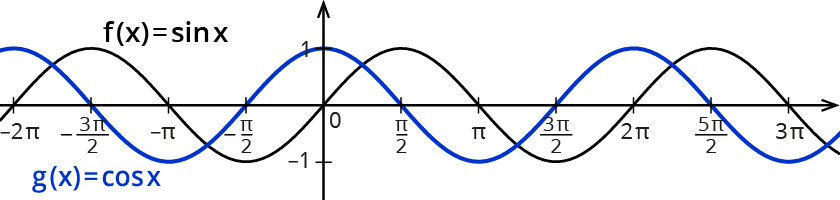
\includegraphics[scale=0.7]{img/sin_cos_2.png}
    \end{center}
    \begin{itemize}
        \item Known as periodic functions: output values repeat in cycles
              \begin{itemize}
                  \item Period: how long it takes to complete a full cycle
                  \item Frequency: inverse of period (i.e.\ portion of period
                        per unit in x-axis)
                  \item Amplitude: highest value from reference value, e.g.\
                        mean, origin, etc. (in sin/cos measured from origin: 1)
              \end{itemize}
    \end{itemize}
\end{frame}

\begin{frame}{Transformer Basics}{Answer c) (i) (2)}
    \begin{itemize}
        \item The construction of positional embeddings only depends on
              hyperparameters $n$ and $d$, so the resulting embedding for
              position $k$ is the same no matter the input sequence.
        \item This is something we want, as these embeddings should
              encode positional information independently of factors such
              as input sequence length.
        \item The $i$-th row of the following matrix thus contains the
              $i$-th positional embedding:
              \begin{center}
                  $\begin{matrix}
                          0.000  & 1.000  & 0.000 & 1.000 \\
                          0.841  & 0.540  & 0.032 & 1.000 \\
                          0.909  & -0.416 & 0.063 & 0.998 \\
                          0.141  & -0.990 & 0.095 & 0.996 \\
                          -0.757 & -0.654 & 0.126 & 0.992
                      \end{matrix}$
              \end{center}
        \item The vectors are not large, as each element in this matrix is
              close to zero, because the output of $\sin$/$\cos$ functions is
              in the range $[-1,1]$.
    \end{itemize}
\end{frame}

\begin{frame}{Transformer Basics}{Answer c) (i) (3)}
    \begin{itemize}
        \item Given that in the original transformer we \emph{add} these
              PEs to input embeddings, we don't want PEs to be large.
        \item The translation that we apply to token embeddings via this
              sum should be large enough to distinguish the same token
              embeddings (which should encode semantics) when used in
              different positions, but not too large that the position
              information becomes a stronger signal to the model than the
              semantics in the input sequence.
        \item In addition, large positional vectors could introduce issues
              during training, such as large gradients that are mostly
              influenced by the position information, or similar issues
              that the model may deal with by making token embeddings
              small enough that they are too constrained to encode
              semantic information well.
        \item All of this depends on operation used to combine token
              embeddings with PEs, e.g.\ different with concatenation.
    \end{itemize}
\end{frame}

\begin{frame}{Transformer Basics}{Question c) (ii)}
    \begin{itemize}
        \item The multiplying factor to $k$ in the argument of the $\sin$/$\cos$
              functions above is known as its frequency.
        \item Given a fixed frequency, i.e.\ using a fixed value of $d, n, i$,
              what happens to the value given by the $\sin$/$\cos$ functions as
              we increase the values of $k$?
        \item What will the features of such vectors look like as a result?
    \end{itemize}
\end{frame}

\begin{frame}{Transformer Basics}{Answer c) (ii) (1)}
    \begin{itemize}
        \item Since the frequency depends on $n,d,i$, each column of our PE
              matrix is a sin/cos function with a fixed frequency.
        \item If we look at each column as we increase values of $k$,
              i.e.\ across rows, we see that elements change values as
              we traverse the $\sin$/$\cos$ (the values of the lasts
              columns also change, but this is less clear due to
              rounding).
    \end{itemize}
    {\scriptsize
    \begin{center}
        $\begin{matrix}
                0.000  & 1.000  & 0.000 & 1.000 & 0.000 & 1.000 & 0.000 & 1.000 & 0.000 & 1.000 \\
                0.841  & 0.5409 & 0.158 & 0.987 & 0.025 & 1.000 & 0.004 & 1.000 & 0.001 & 1.000 \\
                0.909  & -0.416 & 0.312 & 0.95  & 0.05  & 0.999 & 0.008 & 1.000 & 0.001 & 1.000 \\
                0.141  & -0.990 & 0.458 & 0.889 & 0.075 & 0.997 & 0.012 & 1.000 & 0.002 & 1.000 \\
                -0.757 & -0.654 & 0.592 & 0.806 & 0.100 & 0.995 & 0.016 & 1.000 & 0.003 & 1.000 \\
                -0.959 & 0.284  & 0.712 & 0.702 & 0.125 & 0.992 & 0.020 & 1.000 & 0.003 & 1.000 \\
                -0.279 & 0.960  & 0.814 & 0.581 & 0.150 & 0.989 & 0.024 & 1.000 & 0.004 & 1.000 \\
                0.657  & 0.754  & 0.895 & 0.445 & 0.175 & 0.985 & 0.028 & 1.000 & 0.004 & 1.000 \\
                0.989  & -0.146 & 0.954 & 0.298 & 0.200 & 0.980 & 0.032 & 0.999 & 0.005 & 1.000 \\
                0.412  & -0.911 & 0.99  & 0.144 & 0.224 & 0.975 & 0.036 & 0.999 & 0.006 & 1.000
            \end{matrix}$
    \end{center}
    }
    \begin{itemize}
        \item I.e., values in each column vary according to $\sin$/$\cos$.
    \end{itemize}
\end{frame}

\begin{frame}{Transformer Basics}{Answer c) (ii) (2)}
    \begin{itemize}
        \item For uneven values of $i$, we see that values start at $1$
              and decrease as $k$ increases (cosine)
        \item For even values of $k$, we see values increase from $0$ (sine).
        \item This allows us to create vectors with different values for
              contiguous features, i.e.\ vectors that are distinct from
              one another, which is a good thing, because we want \emph{each} of
              them to encode a \emph{different} position, and these vectors are
              not learned.
        \item We discuss the relation between $i$ and $k$, i.e.\ rows and
              columns in the PE matrix, further in the next question.
    \end{itemize}
\end{frame}

\begin{frame}{Transformer Basics}{Question c) (iii)}
    \begin{itemize}
        \item The frequency discussed above is defined as the inverse to the
              period of the function as follows:
              \begin{align*}
                  period = \frac{2\pi}{freq}
              \end{align*}
        \item The period of a function refers to how long it takes to complete a
              full cycle (after which they start to repeat themselves).
        \item In other words, its horizontal stretch.
        \item Using the values for $d$ and $n$ given above, compute the periods
              for different values of $i$.
        \item How do these periods relate to each other?
        \item And what happens to the value of a given element of $i$ for
              different values of $k$?
    \end{itemize}
\end{frame}

\begin{frame}{Transformer Basics}{Answer c) (iii) (1)}
    \begin{itemize}
        \item An example of how a sine function changes with increasing
              frequencies is shown below (higher freq. $\rightarrow$ shorter period).
              \begin{center}
                  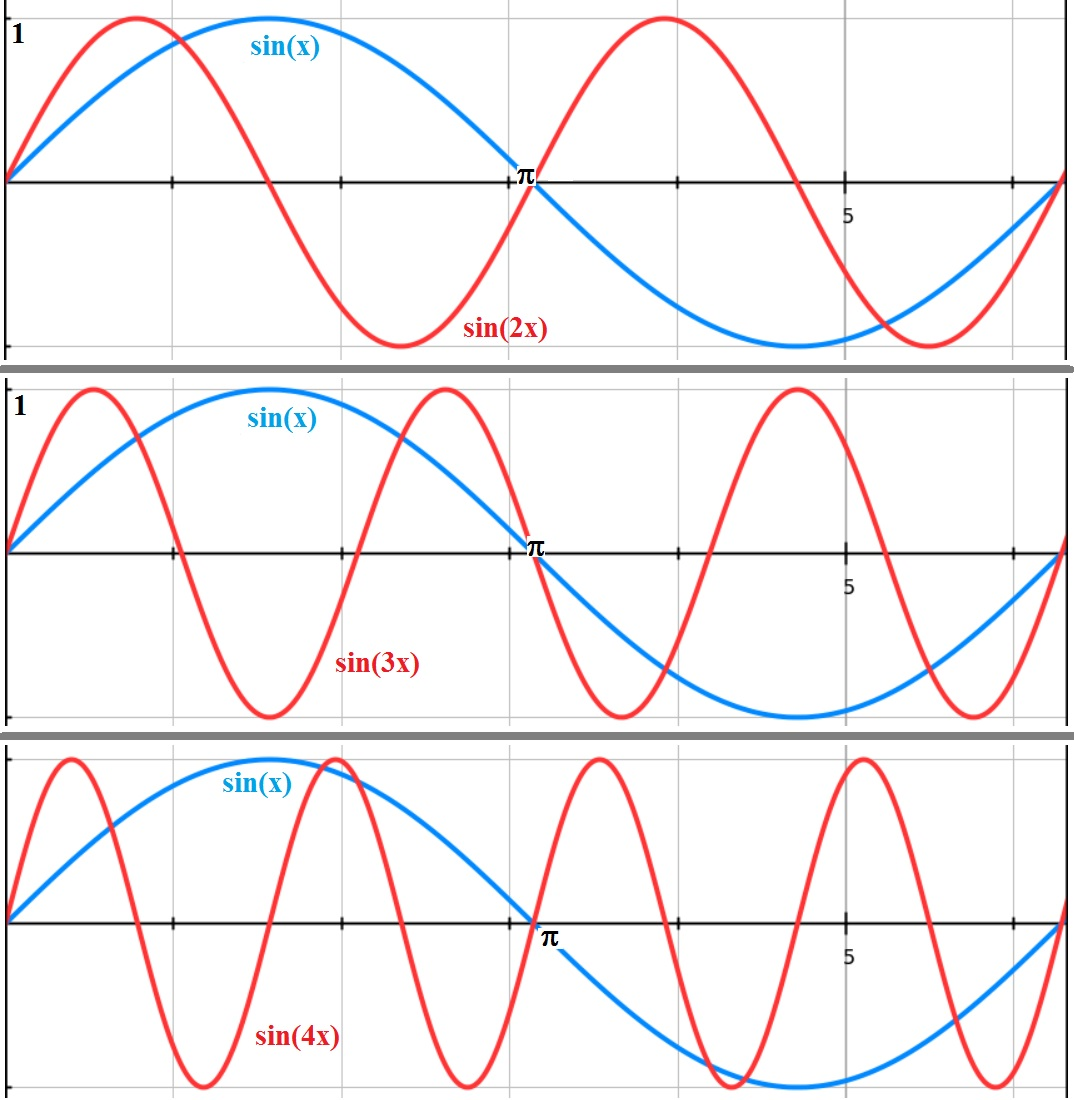
\includegraphics[scale=0.3]{img/sinuscosinus_10.jpg}
              \end{center}
        \item The columns in our PE matrix change following such patterns.
        \item The higher the values of $i$, the lower the frequency and
              the higher the period of these functions.
        \item For example, for the values above, we have for
              $i = [0, 1, 2, 3]$ the corresponding periods
              $[6.28, 198.70, 6283.185, 198691.76]$.
        \item With higher periods, the values across different rows
              (values of $k$) change more slowly.
        \item Thus, the rate of change for a given feature decreases with
              increasing values of $i$ and we get more distinct features
              across different values of $k$ (input positions) and across
              different values of $i$ (positional embedding features).
        \item This allows this non-parametric approach to use vectors
              that are distinct from one another and each encode a
              different position from 1 to some maximum input length.

        \item Overall, this non-parametric approach for obtaining
              positional embeddings is still useful for learning absolute
              position embeddings (APE), but other variants exist.
              BERT and GPT-3 use learned embeddings that encode APEs.
        \item The T5 model learns relative positional embeddings with an
              approach known as \emph{relative bias}, and more recent
              models like PaLM and LLaMa use an approach called
              \emph{rotary}, where they apply rotations to the query and
              key embeddings that are proportional to the absolute
              positions they want to encode.
        \item There are
              \href{https://arxiv.org/pdf/2305.19466.pdf}{studies} that
              look into the differences of such approaches, and some
              \href{https://aclanthology.org/2022.findings-emnlp.99.pdf}{works}
              have suggested that causal language models do not require
              positional embeddings, but still learn positional
              information, which makes sense given the causal approach
              to training and predicting that these models rely on.
    \end{itemize}
\end{frame}

\begin{frame}{Transformer Basics}{Answer c) (iii) (2)}
    \begin{itemize}
        \item The columns, i.e.\ features, in our PE matrix change following
              such patterns.
        \item The higher the values of $i$, the lower the frequency and
              the higher the period of these functions.
        \item For example, for the values above, we have for
              $i = [0, 1, 2, 3]$ the corresponding periods
              $[6.28, 198.70, 6283.185, 198691.76]$.
        \item With higher periods, the values that the same feature (column) in
              our PE matrix takes across different rows (i.e.\ values of $k$)
              change more slowly.
        \item So, the rate of change for a given feature decreases with
              increasing values of $i$ and we get more distinct features
              across different values of $k$ (i.e.\ rows, input positions) and
              across different values of $i$ (i.e.\ columns, positional
              embedding features).
        \item Thus, this (non-parametric) approach uses PE vectors
              that are distinct from one another, each encoding a
              different position from 1 to MAX INPUT LENGTH.
    \end{itemize}
\end{frame}

\begin{frame}{Transformer Basics}{Answer c) (iii) (3)}
    \begin{itemize}
        \item Overall, this non-parametric approach for obtaining
              positional embeddings is still useful for learning absolute
              position embeddings (APE), but other variants exist.
        \item BERT and GPT-3 use learned embeddings that encode APEs.
        \item The T5 model learns relative positional embeddings with an
              approach known as \emph{relative bias}, and more recent
              models like PaLM and LLaMa use an approach called
              \emph{rotary}, where they apply rotations to the query and
              key embeddings that are proportional to the absolute
              positions they want to encode.
        \item There are
              \href{https://arxiv.org/pdf/2305.19466.pdf}{\textcolor{blue}{\underline{studies}}}
              that look into the differences of such approaches, and some
              \href{https://aclanthology.org/2022.findings-emnlp.99.pdf}{\textcolor{blue}{\underline{works}}}
              have suggested that causal language models do not require
              positional embeddings, but still learn positional
              information, which makes sense given the causal approach
              to training and predicting that these models rely on.
    \end{itemize}
\end{frame}

\begin{frame}{Thinking about Perplexity}{Question a)}
    \begin{itemize}
        \item For some random variable $X$, entropy $H(X)$ is defined as
              follows:
              \begin{align}
                  H(x) = -\sum_{x\in X} p(x)\log p(x)
              \end{align}
        \item Say $X$ is the number shown when you toss a fair die.
        \item What is the entropy of $X$?
        \item Use $\log$ base 2 throughout.
    \end{itemize}
\end{frame}

\begin{frame}{Thinking about Perplexity}{Answer a) (1)}
    \begin{itemize}
        \item We have $p(X = i) = \frac{1}{6}$ so that:
              \begin{align*}
                  H(x) = -\sum_{x=1}^6 \frac{1}{6}\log_2\left(\frac{1}{6}\right) \approx 2.58
              \end{align*}
        \item Entropy is a concept from information theory.
        \item We use this definition to define a bit: the entropy of a
              \emph{binary} random variable that takes values 0 or 1 with equal
              probability.
        \item We say we have gained 1 bit of information when the value of such
              a variable becomes known.
        \item When we define entropy using the natural logarithm (we can define it
              using any logarithm), we call such a unit of information a \emph{nat}.
    \end{itemize}
\end{frame}

\begin{frame}{Thinking about Perplexity}{Answer a) (2)}
    \begin{itemize}
        \item A more general intuition about entropy, and one commonly used in
              NLP, is what it tells us about the distribution represented by
              some random variable.
        \item Specifically, the higher the entropy, the more uniform the
              distribution.
        \item This is because the probability mass is distributed more evenly
              across the entire distribution, similar to how then physical
              entropy of a gas always increases to fill up the space it is
              contained in.
    \end{itemize}
\end{frame}

\begin{frame}{Thinking about Perplexity}{Question b)}
    \begin{itemize}
        \item Following a), perplexity is defined as $2^{H(x)}$.
        \item Compute the perplexity of the result you obtained in a).
        \item Can you interpret the result?
        \item How does this expression relate to how we compute perplexity in
              code?
    \end{itemize}
\end{frame}

\begin{frame}{Thinking about Perplexity}{Answer b)}
    \begin{itemize}
        \item We have:
              \begin{align*}
                  ppl(x) = 2^{\left(-\sum_{x=1}^6 \frac{1}{6}\log_2\left(\frac{1}{6}\right)\right)} = 6
              \end{align*}
        \item This is the number of possible values our random variable can
              take.
        \item This is why, in the context of evaluating language models,
              perplexity can be interpreted as the number of possible next words
              given a sequence, often referred to as \emph{branching factor}
              (see Jurafsky Section 3.2.1).
        \item In general, we can use any base for the logarithm when
              computing entropy, but we need to use that same base to compute
              perplexity.
        \item In code, we usually use $\ln$, which is why we use the exponential
              function to compute perplexity.
    \end{itemize}
\end{frame}

\begin{frame}{Thinking about Perplexity}{Question c)}
    \begin{itemize}
        \item In NLP, we are interested in the entropy of sequences.
              Say $X$ is now a random variable over all possible sequences of
              length $n$ over some language $L$.
        \item Write the expression to compute this entropy.
        \item How would you compute the average entropy per word in such a
              sequence?
    \end{itemize}
\end{frame}

\begin{frame}{Thinking about Perplexity}{Answer c)}
    \begin{itemize}
        \item We have:
              \begin{align*}
                  H(w_1,w_2,\ldots,w_n) = -\sum_{w_{1:n}\in L} p(w_{1:n})\log p(w_{1:n})
              \end{align*}
        \item The average entropy per word in the sequence, also known as
              \emph{entropy rate}, is given by:
              \begin{align*}
                  H(w_1,w_2,\ldots,w_n) = -\frac{1}{n}\sum_{w_{1:n}\in L} p(w_{1:n})\log p(w_{1:n})
              \end{align*}
        \item Note that we overload $H(x)$ to also represent entropy rate.
    \end{itemize}
\end{frame}

\begin{frame}{Thinking about Perplexity}{Question d)}
    \begin{itemize}
        \item In the context of language models, $p$ is the distribution over
              some natural language $L$, and we don't have access to this
              distribution.
        \item Instead, we learn an estimate $m$ of this distribution from data.
        \item In such a context, the concept of \emph{cross-entropy} $H(p,m)$ is
              suitable.
        \item It is defined as the sum of $p(x)$ for all $x\in X$ weighted by
              their corresponding $\log$ probabilities according to $m$.
        \item Write the cross-entropy \emph{rate} for a sequence of length $n$.
    \end{itemize}
\end{frame}

\begin{frame}{Thinking about Perplexity}{Answer d)}
    \begin{itemize}
        \item The cross-entropy of some model $m$ of $p$ is defined as:
              \begin{align*}
                  H(w_1,w_2,\ldots,w_n) = -\frac{1}{n}\sum_{w_{1:n}\in L} p(w_{1:n})\log m(w_{1:n})
              \end{align*}
        \item The intuition here is that we draw sequences from $p$, but we
              weigh them by their probability according to model $m$.
        \item In other words, this expectation (average information, i.e.\
              entropy) is according to $m$.
        \item From a training perspective, $p$ is typically the target
              distribution that we want to learn with model $m$.
        \item In the case of entropy of sequences of text, you can think of $m$
              as the softmax distribution of a language model you are training,
              and $p$ the target distribution set by self-supervision (all the
              mass on a single word in the vocabulary).
    \end{itemize}
\end{frame}

\begin{frame}{Thinking about Perplexity}{Question e)}
    \begin{itemize}
        \item It can be shown that the cross-entropy of a language can be
              approximated by the following expression:
              \begin{align}
                  H(W) = -\frac{1}{N} \log p(w_1,w_2,\ldots,w_N)
              \end{align}
              where $N$ is a sufficiently large number and $w_i$ are words in
              that language.
        \item As seen in question (b), perplexity is formally defined as
              $ppl(W) = 2^{H(W)}$, where $W$ is $w_1, w_2, \ldots, w_N$, and we
              define entropy using log base 2.
        \item Use this approximation of cross-entropy given above to compute the
              expression for perplexity given in the lecture.
        \item What does this expression say about how we evaluate a language
              model by computing perplexity on a held-out corpus?
    \end{itemize}
\end{frame}

\begin{frame}{Thinking about Perplexity}{Answer e)}
    \begin{itemize}
        \item We proceed as follows:
              \begin{align*}
                  ppl(W) & = 2^{H(W)}                                                                   \\
                         & = 2^{\left(-\frac{1}{N} \log p(W)\right)} &  & (\text{apply log properties}) \\
                         & = p(W)^{-\frac{1}{N}}.
              \end{align*}
        \item The approximation given in this question shows us not only how
              perplexity is related to entropy, but it also explains what we are
              doing when we compute the perplexity of a held-out validation
              corpus:
              \begin{itemize}
                  \item We are estimating the cross-entropy of the entire
                        language, where $m$ is our language model and $p$ the
                        true distribution of the language.
              \end{itemize}
        \item Recall from machine learning courses, that cross-entropy is
              equivalent to log-loss, which explains why we typically apply the
              exponential function to our loss value to get perplexity in code
              ($\exp$ because we use $\ln$).
    \end{itemize}
\end{frame}

\begin{frame}{Thinking about Perplexity}{Takeaway 1 of 3}
    \begin{itemize}
        \item Since we typically train language models with the cross-entropy
              loss, a.k.a.\ log loss, and we use $\ln$ to compute logarithms in
              code, applying the $\exp$ function to our loss gives us
              perplexity, because $ppl = e^{H(W)}$ according to Eq. 1 in the
              task description.
    \end{itemize}
    \begin{align*}
        H(x) = -\sum_{x\in X} p(x)\log p(x)
    \end{align*}
\end{frame}

\begin{frame}{Thinking about Perplexity}{Takeaway 2 of 3}
    \begin{itemize}
        \item The definition of perplexity from the lecture, i.e.\
              $p(W)^{\frac{1}{N}}$, is related to the definition of perplexity
              from information theory, i.e.\ $2^{H(W)}$ assuming log base 2, via
              the way to approximate the entropy of a language described in
              Eq. 2 in the task description.
    \end{itemize}
    \begin{align*}
        H(W) = -\frac{1}{N} \log p(w_1,w_2,\ldots,w_N)
    \end{align*}
\end{frame}

\begin{frame}{Thinking about Perplexity}{Takeaway 3 of 3}
    \begin{itemize}
        \item The point above suggests that when computing the perplexity of a
              language model on a held-out corpus, we are estimating the
              cross-entropy of the entire language used in the validation
              corpus.
              Since the larger the $N$ in Eq. 2, the better the estimate, we
              want to use a large enough validation corpus.
    \end{itemize}
    \begin{align*}
        H(W) = -\frac{1}{N} \log p(w_1,w_2,\ldots,w_N)
    \end{align*}
\end{frame}

\end{document}
